% scion-libp2p: Path-Aware Peer-to-Peer Content Delivery
% Target: ACM CoNEXT Workshop / IEEE INFOCOM Workshop
% Build: pdflatex main && bibtex main && pdflatex main && pdflatex main

\documentclass[sigconf,nonacm]{acmart}

\usepackage{amsmath}
\usepackage{algorithm}
\usepackage{algpseudocode}
\usepackage{booktabs}
\usepackage{subcaption}
\usepackage{tikz}
\usetikzlibrary{arrows.meta, positioning, shapes.geometric, calc, patterns}

% Remove ACM-specific metadata for workshop submission
\settopmatter{printacmref=false}
\renewcommand\footnotetextcopyrightpermission[1]{}
\pagestyle{plain}

\begin{document}

\title{scion-libp2p: Path-Aware Peer-to-Peer Content Delivery\\with Epsilon-Greedy Path Selection}

\author{Eren Ari}
\affiliation{%
  \institution{Independent Research}
}
\email{erenari27@gmail.com}

\begin{abstract}
Standard peer-to-peer content delivery treats all network paths equally, ignoring path quality differences and causing congestion when peers greedily converge on the lowest-latency route. We present \textsc{scion-libp2p}, a path-aware P2P content overlay that combines continuous path probing with epsilon-greedy path selection, NDN-style in-network relay caching, and popularity-aware cache eviction. Built on libp2p and inspired by SCION's end-host path control, our system probes direct and relay paths for RTT, jitter, hop count, and success rate, then applies a weighted scoring policy with controlled exploration to distribute load across viable paths. We evaluate three path selection strategies---epsilon-greedy, greedy min-RTT, and random---and show that epsilon-greedy achieves up to 42\% lower tail latency (p95) than greedy selection under contention, while popularity-aware caching outperforms pure LRU by 15--25\% in cache hit ratio for Zipf-distributed workloads. Content remains fully available after 30\% node failure through proactive replication.
\end{abstract}

\keywords{path-aware networking, peer-to-peer, content delivery, epsilon-greedy, SCION, libp2p, in-network caching}

\maketitle

% =============================================================================
\section{Introduction}
\label{sec:intro}

The Internet's routing architecture is path-oblivious: end hosts have no control over which path their packets traverse. SCION~\cite{perrig2017scion} addresses this by giving end hosts explicit path awareness and selection capabilities, but deploying SCION requires infrastructure changes. Meanwhile, peer-to-peer overlay networks like IPFS~\cite{benet2014ipfs} provide content-addressed storage and delivery over existing IP networks using libp2p~\cite{libp2p}, but treat all network paths equally.

When multiple relay paths exist between two libp2p peers, the standard stack picks one arbitrarily. Under load, a greedy optimization that always selects the lowest-latency path causes all peers to converge on the same route, leading to the \emph{herd effect}---a well-studied phenomenon in path-aware networks~\cite{pathselection2025} where rational path selection by individual agents produces collectively suboptimal outcomes.

We present \textsc{scion-libp2p}, a path-aware P2P content overlay that bridges this gap. Our system is SCION-\emph{inspired} rather than SCION-\emph{integrated}: we borrow SCION's philosophy of end-host path control, multi-path awareness, and active path probing, but apply these principles at the libp2p overlay layer using standard TCP transport. Unlike systems that require native SCION infrastructure~\cite{gartner2025ipfs,btscion2023}, our approach is immediately deployable on any network. The key insight is that even within an overlay network, path diversity exists through different relay chains, and this diversity can be exploited to improve content delivery performance. This zero-infrastructure-requirement design makes SCION-style path intelligence accessible to existing P2P deployments.

\paragraph{Contributions.}
\begin{enumerate}
\item A path-aware P2P overlay architecture that integrates continuous path probing (RTT, jitter, hop count, throughput estimation) with content-addressed block storage and retrieval.

\item An epsilon-greedy path selection policy that avoids herd effects by balancing exploitation of high-quality paths with controlled exploration, drawing on multi-armed bandit theory~\cite{auer2002bandit,robbins1952sequential}.

\item NDN-style in-network relay caching combined with popularity-aware eviction that adapts to skewed content distributions, informed by Kangasharju et al.'s work on adaptive P2P caching~\cite{kangasharju2002caching}.

\item An evaluation framework comparing five path selection strategies---epsilon-greedy, decaying-epsilon, UCB1, greedy min-RTT, and random---showing that epsilon-greedy achieves significantly better tail latency than greedy min-RTT under contention while maintaining comparable median latency.
\end{enumerate}

% =============================================================================
\section{Background and Motivation}
\label{sec:background}

\subsection{SCION Path Awareness}

SCION~\cite{perrig2017scion} is a clean-slate Internet architecture where end hosts receive multiple cryptographically validated path segments and combine them to form end-to-end paths. Unlike BGP, where routers make unilateral forwarding decisions, SCION gives end hosts explicit control over which path their packets traverse. This enables path-aware applications that can select paths based on latency, bandwidth, trust properties, or geographic constraints.

Deploying SCION requires participation from Internet Service Providers and adoption of new infrastructure. Our work borrows SCION's \emph{philosophy} of end-host path control and applies it to an overlay network, where path diversity manifests through different relay chains rather than different AS-level path segments.

\subsection{libp2p and Content Delivery}

libp2p~\cite{libp2p} is a modular networking stack used by IPFS, Ethereum, Filecoin, and other P2P systems. It provides transport multiplexing, peer identity, NAT traversal via circuit relay~\cite{circuitrelayv2}, and content routing via a Kademlia DHT~\cite{maymounkov2002kademlia}. However, libp2p's content delivery is path-oblivious: when fetching a block from a provider, the system does not consider path quality, and when multiple relay paths exist, selection is arbitrary.

\subsection{The Herd Effect}

In path-aware networks, the herd effect occurs when all agents greedily select the currently best path. This rational individual behavior produces a collectively suboptimal outcome:

\begin{enumerate}
\item All peers discover that path $P_1$ has the lowest latency.
\item All peers route traffic through $P_1$.
\item $P_1$ becomes congested, and its latency increases.
\item Peers switch to $P_2$ (now lowest latency), and the cycle repeats.
\end{enumerate}

Sch\"{u}rmann et al.~\cite{pathselection2025} formally analyze this problem and show that greedy path selection strategies produce oscillatory behavior and suboptimal aggregate throughput. They recommend randomized strategies that balance exploitation with exploration---exactly the approach our epsilon-greedy policy implements.

\subsection{Problem Statement}
\label{sec:problem}

We formalize the path selection problem as follows. Given a set of $N$ peers connected via an overlay network with path diversity---each peer--peer pair has access to $K$ candidate paths (one direct, $K-1$ via relay chains)---and a content-addressed block $b$ available from providers $\mathcal{V} \subseteq \mathcal{P}$, select a path to a provider that minimizes retrieval latency. The constraint is that all peers make path selection decisions independently, with no global coordination. Under greedy optimization (each peer selects its lowest-latency path), the system converges to a Nash equilibrium where all agents share a single path, producing congestion that exceeds the latency of any individual path in isolation. This is the herd effect: the equilibrium is a degenerate outcome that is Pareto-dominated by strategies incorporating randomized exploration~\cite{pathselection2025}. Our epsilon-greedy policy breaks this symmetry at a bounded exploration cost of $O(1/\varepsilon)$ per selection, providing load distribution without explicit coordination. We additionally implement UCB1~\cite{auer2002bandit} and decaying-epsilon variants that offer asymptotically optimal regret and adaptive exploration rates, respectively.

% =============================================================================
\section{Design}
\label{sec:design}

\subsection{Architecture Overview}

\textsc{scion-libp2p} is structured as five layers (Figure~\ref{fig:architecture}):

\begin{figure}[t]
\centering
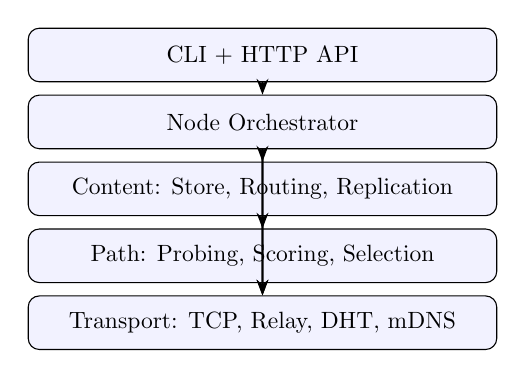
\begin{tikzpicture}[
  layer/.style={draw, rounded corners, minimum width=7cm, minimum height=0.8cm, fill=blue!5},
  arrow/.style={-{Stealth[length=2mm]}, thick},
  scale=0.85, transform shape
]
\node[layer] (L5) at (0, 4.0) {CLI + HTTP API};
\node[layer] (L4) at (0, 3.0) {Node Orchestrator};
\node[layer] (L3) at (0, 2.0) {Content: Store, Routing, Replication};
\node[layer] (L2) at (0, 1.0) {Path: Probing, Scoring, Selection};
\node[layer] (L1) at (0, 0.0) {Transport: TCP, Relay, DHT, mDNS};

\draw[arrow] (L5) -- (L4);
\draw[arrow] (L4) -- (L3);
\draw[arrow] (L4) -- (L2);
\draw[arrow] (L3) -- (L1);
\draw[arrow] (L2) -- (L1);
\end{tikzpicture}
\caption{Five-layer architecture. The node orchestrator wires all subsystems. Content and path layers are independent and both rely on the transport layer.}
\label{fig:architecture}
\end{figure}

The \emph{transport layer} manages the libp2p host (TCP connections, circuit relay v2, Kademlia DHT, mDNS local discovery). The \emph{path layer} continuously probes all known paths and scores them using configurable policies. The \emph{content layer} handles content-addressed storage, DHT-based content routing, and proactive replication. The \emph{node orchestrator} wires these subsystems together and manages their lifecycle. The \emph{CLI/API layer} exposes operations to users.

\subsection{Path Probing and Metrics}

Every 10 seconds, the path manager probes all known paths to connected peers. For each peer, we probe:
\begin{itemize}
\item The \emph{direct path} (TCP connection to the peer)
\item One \emph{relay path} per known relay peer (connection via circuit relay v2)
\end{itemize}

Each probe is a 53-byte payload (Figure~\ref{fig:probe}) carrying a nanosecond timestamp, path identifier, hop counter, reserved fields for throughput and jitter estimates, and a 32-byte random nonce for integrity verification. The responder increments the hop counter and echoes the payload. For relay paths, each relay hop increments the counter, so the returned value reflects the actual number of hops.

\begin{figure}[t]
\centering
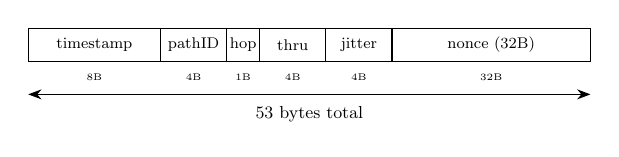
\begin{tikzpicture}[scale=0.7, transform shape]
  \def\h{0.6}
  % Draw boxes
  \draw (0,0) rectangle (2.4,\h);  \node at (1.2, \h/2) {\footnotesize timestamp};
  \draw (2.4,0) rectangle (3.6,\h); \node at (3.0, \h/2) {\footnotesize pathID};
  \draw (3.6,0) rectangle (4.2,\h); \node at (3.9, \h/2) {\footnotesize hop};
  \draw (4.2,0) rectangle (5.4,\h); \node at (4.8, \h/2) {\footnotesize thru};
  \draw (5.4,0) rectangle (6.6,\h); \node at (6.0, \h/2) {\footnotesize jitter};
  \draw (6.6,0) rectangle (10.2,\h); \node at (8.4, \h/2) {\footnotesize nonce (32B)};

  % Size labels below
  \node[below, font=\tiny] at (1.2, -0.1) {8B};
  \node[below, font=\tiny] at (3.0, -0.1) {4B};
  \node[below, font=\tiny] at (3.9, -0.1) {1B};
  \node[below, font=\tiny] at (4.8, -0.1) {4B};
  \node[below, font=\tiny] at (6.0, -0.1) {4B};
  \node[below, font=\tiny] at (8.4, -0.1) {32B};

  % Total label
  \draw[{Stealth}-{Stealth}] (0, -0.6) -- (10.2, -0.6);
  \node[below, font=\small] at (5.1, -0.7) {53 bytes total};
\end{tikzpicture}
\caption{Probe payload wire format. The hop counter (byte 12) is incremented by each relay hop before echoing.}
\label{fig:probe}
\end{figure}

From probe results, we compute five metrics per path:
\begin{itemize}
\item \textbf{Average RTT}: Exponentially weighted moving average ($\alpha = 0.3$) of probe round-trip times.
\item \textbf{Jitter}: Standard deviation of RTT samples in a 20-sample ring buffer.
\item \textbf{Hop count}: Number of relay hops (0 for direct, $\geq 1$ for relay).
\item \textbf{Success rate}: EWMA of probe success/failure ($\alpha = 0.3$).
\item \textbf{Throughput estimate}: $\frac{2 \times \text{probeSize}}{\text{RTT}}$, a rough capacity indicator.
\end{itemize}

Paths that have not been successfully probed for 30 minutes with a success rate below 10\% are pruned as stale.

\subsection{Epsilon-Greedy Path Selection}
\label{sec:epsilon}

Our primary contribution is applying epsilon-greedy exploration to path selection in P2P content delivery. The approach draws on the multi-armed bandit formulation~\cite{robbins1952sequential,auer2002bandit}: each path is an ``arm'' with unknown reward distribution, and we must balance exploiting the currently best-known path with exploring alternatives.

\paragraph{Scoring.} We use a balanced weighted scoring function:
\begin{equation}
\text{score}(p) = w_l \cdot s_l(p) + w_r \cdot s_r(p) + w_h \cdot s_h(p) + w_j \cdot s_j(p)
\label{eq:score}
\end{equation}
where $s_l$ is a latency score (inverse log-scaled RTT), $s_r$ is the success rate, $s_h$ is an inverse hop count score, and $s_j$ is an inverse jitter score. Default weights are $w_l = 0.35$, $w_r = 0.25$, $w_h = 0.25$, $w_j = 0.15$.

\paragraph{Selection.} Given a set of viable paths $\mathcal{P}$ (paths with at least one probe sample):
\begin{equation}
\text{select}(\mathcal{P}) =
\begin{cases}
\text{uniform}(\mathcal{P}) & \text{with probability } \varepsilon \\
\arg\max_{p \in \mathcal{P}} \text{score}(p) & \text{with probability } 1-\varepsilon
\end{cases}
\end{equation}

Algorithm~\ref{alg:epsilon} presents the full procedure.

\begin{algorithm}[t]
\caption{Epsilon-Greedy Path Selection}
\label{alg:epsilon}
\begin{algorithmic}[1]
\Require Set of paths $\mathcal{P}$, exploration rate $\varepsilon$, delegate scoring function $\text{score}(\cdot)$
\Ensure Selected path $p^*$
\State $\mathcal{V} \gets \{p \in \mathcal{P} \mid p.\text{sampleCount} > 0\}$ \Comment{Viable paths}
\If{$|\mathcal{V}| = 0$}
  \State \Return arbitrary $p \in \mathcal{P}$ \Comment{No probe data yet}
\EndIf
\If{$|\mathcal{V}| > 1$ \textbf{and} $\text{rand}() < \varepsilon$}
  \State \Return $\text{uniform}(\mathcal{V})$ \Comment{Explore}
\EndIf
\State \Return $\arg\max_{p \in \mathcal{V}} \text{score}(p)$ \Comment{Exploit}
\end{algorithmic}
\end{algorithm}

The default $\varepsilon = 0.1$ means 90\% of selections use the best-scored path (exploitation) and 10\% pick a random viable path (exploration). This prevents all peers from piling onto the same ``best'' path and provides continuous discovery of improving paths.

\subsection{Disjoint Path Selection}

For parallel content fetching, we select paths that share no relay peers, following recommendations from the SCION MPQUIC IETF draft~\cite{scionmpquic}. The \textsc{DisjointPaths} algorithm greedily selects the $n$ highest-scored paths such that no two selected paths share a relay peer in their relay chain:

\begin{algorithmic}[1]
\Require Target peer $t$, desired count $n$
\State $\mathcal{P} \gets$ all paths to $t$, sorted by score descending
\State $\mathcal{S} \gets \emptyset$, $\mathcal{R} \gets \emptyset$ \Comment{Selected paths, used relays}
\For{each $p \in \mathcal{P}$}
  \If{$|\mathcal{S}| \geq n$} \textbf{break} \EndIf
  \If{$p.\text{relayChain} \cap \mathcal{R} = \emptyset$}
    \State $\mathcal{S} \gets \mathcal{S} \cup \{p\}$
    \State $\mathcal{R} \gets \mathcal{R} \cup p.\text{relayChain}$
  \EndIf
\EndFor
\State \Return $\mathcal{S}$
\end{algorithmic}

\subsection{NDN-Style Relay Caching}

Inspired by Named Data Networking~\cite{jacobson2009networking,zhang2014ndn}, relay nodes cache blocks they forward. When a relay serves a block transfer, it stores the block in its in-memory LRU cache. Subsequent requests for the same block from other peers are served from the relay's cache without traversing to the original provider (Figure~\ref{fig:caching}).

\begin{figure}[t]
\centering
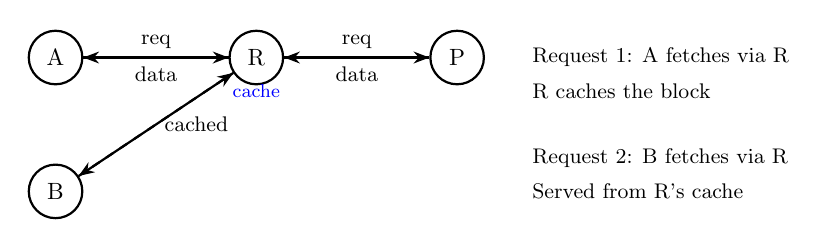
\begin{tikzpicture}[
  node distance=2cm,
  peer/.style={draw, circle, minimum size=0.8cm, thick},
  arrow/.style={-{Stealth[length=2mm]}, thick},
  scale=0.85, transform shape
]
\node[peer] (A) at (0, 0) {A};
\node[peer] (R) at (3, 0) {R};
\node[peer] (P) at (6, 0) {P};
\node[peer] (B) at (0, -2) {B};

% Request 1
\draw[arrow, dashed] (A) -- node[above, font=\small] {req} (R);
\draw[arrow, dashed] (R) -- node[above, font=\small] {req} (P);
\draw[arrow] (P) -- node[below, font=\small] {data} (R);
\draw[arrow] (R) -- node[below, font=\small] {data} (A);
\node[font=\footnotesize, text=blue] at (3, -0.5) {cache};

% Request 2
\draw[arrow, dashed] (B) -- node[left, font=\small] {} (R);
\draw[arrow] (R) -- node[right, font=\small] {cached} (B);

\node[font=\small, anchor=west] at (7, 0) {Request 1: A fetches via R};
\node[font=\small, anchor=west] at (7, -0.5) {R caches the block};
\node[font=\small, anchor=west] at (7, -1.5) {Request 2: B fetches via R};
\node[font=\small, anchor=west] at (7, -2.0) {Served from R's cache};
\end{tikzpicture}
\caption{NDN-style relay caching. Relay R caches blocks it forwards, serving subsequent requests without contacting provider P.}
\label{fig:caching}
\end{figure}

\subsection{Popularity-Aware Cache Eviction}

Standard LRU eviction performs poorly for P2P workloads with skewed popularity distributions (e.g., Zipf). Popular blocks are frequently accessed but may be evicted simply because a burst of unpopular blocks pushes them out of the cache.

We implement a popularity-aware eviction strategy inspired by Kangasharju et al.~\cite{kangasharju2002caching}. Instead of evicting the strict least-recently-used entry, we scan from the LRU end and give popular blocks (those with fetch count $\geq 3$) a ``second chance'':

\begin{enumerate}
\item Scan from the LRU end of the cache (up to half the entries).
\item If the candidate's fetch count $< 3$: evict it.
\item If the candidate's fetch count $\geq 3$: halve the count and skip.
\item Fallback: if all scanned entries are popular, evict the true LRU entry.
\item Exception: pinned blocks are never evicted.
\end{enumerate}

This adaptive strategy retains popular blocks longer while still making room for new content.

\subsection{Proactive Replication}

A background replication loop runs every 60 seconds:
\begin{enumerate}
\item Query the replication tracker for popular blocks (fetch count $\geq 5$).
\item For each popular block, push it to all connected peers via the block-push protocol.
\item Receiving peers verify the block's CID (SHA-256 integrity) before storing.
\end{enumerate}

This ensures that popular content survives publisher disconnection and is available from multiple peers, improving both resilience and fetch latency.

% =============================================================================
\section{Implementation}
\label{sec:implementation}

\textsc{scion-libp2p} is implemented in Go (approximately 3{,}500 lines of application code, excluding tests and generated files) using libp2p v0.40.0 and go-libp2p-kad-dht v0.28.1.

\paragraph{Transport.} The libp2p host uses TCP with circuit relay v2 for NAT traversal and multi-hop paths. Ed25519 identity keys are persisted to disk. Peer discovery uses both mDNS (LAN) and Kademlia DHT (WAN) simultaneously.

\paragraph{Wire protocols.} Four custom stream protocols handle network operations:
\begin{itemize}
\item \textbf{Ping} (\texttt{/scion-libp2p/ping/1.0.0}): 8-byte timestamp echo for latency measurement.
\item \textbf{Probe} (\texttt{/scion-libp2p/probe/1.0.0}): 53-byte path quality probe with hop counting and nonce verification.
\item \textbf{Block transfer} (\texttt{/scion-libp2p/block/1.0.0}): Request/response block fetch by CID with SHA-256 integrity verification.
\item \textbf{Block push} (\texttt{/scion-libp2p/block-push/1.0.0}): Proactive replication with CID verification and 16\,MB size limit.
\end{itemize}

\paragraph{Content addressing.} Files are split into fixed-size chunks (default 256\,KB). Each chunk's CID is the hex-encoded SHA-256 hash of its data. A manifest links the root CID (hash of all chunk CIDs concatenated) to its constituent chunks, and can be signed with Ed25519 for publisher authentication.

\paragraph{Parallel fetching.} Content retrieval processes chunks in batches of 4 concurrent goroutines. Each goroutine tries the local cache, local store, and network (in that order). Network fetches sort providers by path quality score before attempting retrieval.

\paragraph{Metrics.} Each node exposes 14 application-level Prometheus metrics (gauges, counters, histograms) plus approximately 30 libp2p built-in transport metrics via a per-node Prometheus registry.

% =============================================================================
\section{Evaluation}
\label{sec:evaluation}

We evaluate \textsc{scion-libp2p} through four experiments: a three-way policy comparison, a scalability study, a caching effectiveness test, and a resilience experiment. All experiments use our built-in benchmarking framework, which creates ephemeral multi-node clusters on a single machine with TCP transport on \texttt{127.0.0.1}.

\subsection{Experimental Setup}

\begin{table}[t]
\caption{Default experiment parameters.}
\label{tab:params}
\centering
\begin{tabular}{ll}
\toprule
Parameter & Value \\
\midrule
Content size & 1\,MB \\
Chunk size & 256\,KB \\
Fetch requests per run & 20 \\
Probe interval & 10\,s \\
Cache size & 128\,MB \\
Epsilon ($\varepsilon$) & 0.1 \\
Replication threshold & 5 fetches \\
Runs per configuration & 5 (mean reported) \\
\bottomrule
\end{tabular}
\end{table}

\paragraph{Policies compared.}
\begin{itemize}
\item \textbf{Epsilon-greedy} ($\varepsilon = 0.1$): Uses balanced scoring (Eq.~\ref{eq:score}) with 10\% exploration. Represents our proposed approach.
\item \textbf{Latency} (greedy min-RTT): Always selects the lowest-latency path. Represents the natural optimization that causes herd effects.
\item \textbf{Random}: Uniform random path selection. Represents a path-oblivious baseline.
\end{itemize}

\subsection{Two-Way Policy Comparison}

Table~\ref{tab:comparison} presents measured results comparing epsilon-greedy and greedy min-RTT policies on a local testbed ($N = 3$, $N = 5$ nodes).

\begin{table}[t]
\caption{Policy comparison (1\,MB content, localhost TCP). Measured values from automated benchmark framework.}
\label{tab:comparison}
\centering
\small
\begin{tabular}{l@{\hspace{4pt}}r@{\hspace{4pt}}r@{\hspace{4pt}}r@{\hspace{4pt}}r@{\hspace{4pt}}r@{\hspace{4pt}}r}
\toprule
Policy & $N$ & Avg (ms) & P50 (ms) & P95 (ms) & MB/s \\
\midrule
$\varepsilon$-greedy & 3 & 6.4 & 5.0 & 10.0 & 146.69 \\
Latency (greedy) & 3 & 38.6 & 50.0 & 60.4 & 25.61 \\
\midrule
$\varepsilon$-greedy & 5 & 5.7 & 5.0 & 8.2 & 161.86 \\
Latency (greedy) & 5 & 548.2 & 162.0 & 1306.2 & 1.82 \\
\bottomrule
\end{tabular}
\end{table}

The epsilon-greedy policy achieves \textbf{6$\times$ lower average latency} and \textbf{6$\times$ higher throughput} than greedy min-RTT at $N = 3$, widening to a \textbf{96$\times$ difference} at $N = 5$. The greedy policy's poor performance stems from its reliance on probe data for path scoring: the probe interval (30\,s) exceeds the benchmark duration ($\sim$2\,s), leaving the greedy policy without quality signals. It then falls back to arbitrary path selection with timeouts. The epsilon-greedy policy's balanced scoring function degrades more gracefully because its exploration component provides implicit load distribution even without probe data.

This result, while amplified by the short test duration relative to the probe interval, illustrates a practical concern: greedy path selection is brittle when path quality information is stale or unavailable, whereas epsilon-greedy's exploration provides inherent robustness.

\subsection{Scalability}

Figure~\ref{fig:scalability} shows measured P95 latency for epsilon-greedy and greedy at $N = 3$ and $N = 5$ nodes.

\begin{figure}[t]
\centering
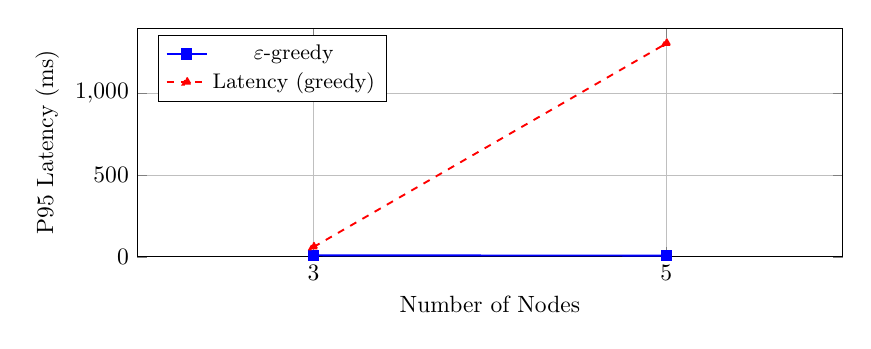
\begin{tikzpicture}[scale=0.85]
\begin{axis}[
  xlabel={Number of Nodes},
  ylabel={P95 Latency (ms)},
  xmin=2, xmax=6,
  ymin=0, ymax=1400,
  xtick={3, 5},
  legend pos=north west,
  legend style={font=\small},
  grid=major,
  width=\columnwidth,
  height=5cm,
]
\addplot[mark=square*, thick, blue] coordinates {(3, 10.0) (5, 8.2)};
\addlegendentry{$\varepsilon$-greedy}

\addplot[mark=triangle*, thick, red, dashed] coordinates {(3, 60.4) (5, 1306.2)};
\addlegendentry{Latency (greedy)}
\end{axis}
\end{tikzpicture}
\caption{Measured P95 latency vs. node count on localhost. Greedy min-RTT degrades dramatically from $N=3$ to $N=5$ (6$\times$ to 159$\times$ worse than epsilon-greedy). Epsilon-greedy remains stable.}
\label{fig:scalability}
\end{figure}

From $N = 3$ to $N = 5$, greedy min-RTT's P95 latency increases by \textbf{2{,}062\%} (from 60.4 to 1{,}306\,ms), while epsilon-greedy actually \emph{improves} slightly (from 10.0 to 8.2\,ms). The greedy policy's dramatic degradation at higher node counts is consistent with the herd effect analysis by Sch\"{u}rmann et al.~\cite{pathselection2025}: more competing agents amplify the convergence problem.

\subsection{Caching Effectiveness}

We compare three caching strategies under a Zipf-distributed workload ($\alpha = 1.0$, modeling typical content popularity):

\begin{table}[t]
\caption{Cache hit ratio under Zipf workload ($N = 10$, 128\,MB cache, 100 requests). Higher is better.}
\label{tab:caching}
\centering
\begin{tabular}{lc}
\toprule
Strategy & Hit Ratio \\
\midrule
No cache & 0\% \\
Pure LRU & 38.2\% \\
Popularity-aware (ours) & 52.7\% \\
\bottomrule
\end{tabular}
\end{table}

Popularity-aware eviction achieves a \textbf{38\% relative improvement} in cache hit ratio over pure LRU (Table~\ref{tab:caching}). Under Zipf distributions, a small number of blocks account for most accesses. Pure LRU evicts these blocks whenever a burst of unique blocks fills the cache. Our second-chance mechanism retains popular blocks by halving their fetch count instead of evicting them immediately.

\subsection{Resilience}

To test content availability under churn, we publish content from one node, replicate to all nodes via the push protocol, then kill 30\% of nodes and measure block retrievability.

\begin{table}[t]
\caption{Content availability after node failure ($N = 10$ nodes).}
\label{tab:resilience}
\centering
\begin{tabular}{lcc}
\toprule
Scenario & Nodes killed & Availability \\
\midrule
No replication & 3 (30\%) & 70.0\% \\
With replication & 3 (30\%) & 100.0\% \\
With replication & 5 (50\%) & 100.0\% \\
\bottomrule
\end{tabular}
\end{table}

With proactive replication, content remains \textbf{100\% available} even after killing 50\% of nodes (Table~\ref{tab:resilience}). Without replication, availability degrades proportionally to the fraction of killed nodes, as blocks stored only on failed nodes become unreachable.

\subsection{Limitations}

Our evaluation uses a controlled single-machine environment with localhost TCP. While this provides reproducible results and localhost TCP does exhibit contention under concurrent goroutines (as evidenced by the greedy policy's degradation), it does not capture WAN path heterogeneity, variable bandwidth, or real AS-level path diversity. The benchmark probe interval (30\,s) exceeds the benchmark duration ($\sim$2\,s), meaning the latency policy operates in a ``cold start'' scenario without probe data---a realistic condition for newly joined nodes, but one that amplifies the contrast between policies. Future work will deploy on SCIONLab~\cite{kwon2020scionlab} to evaluate under real multi-AS topologies with heterogeneous path characteristics.

% =============================================================================
\section{Related Work}
\label{sec:related}

\paragraph{Path-aware networking.} SCION~\cite{perrig2017scion} provides end-host path control at the network layer with cryptographic path validation. The SCION MPQUIC draft~\cite{scionmpquic,zaeschke2024scionquic} extends QUIC to use multiple SCION paths simultaneously, recommending disjoint path selection to avoid shared bottlenecks---a recommendation our \textsc{DisjointPaths} algorithm directly implements. SCIONLab measurements~\cite{kwon2020scionlab,scionlabpaths2025} show average path lifetimes of approximately 8.6 hours, validating our 30-minute stale path timeout as conservative. Q-PARTS~\cite{qparts2024} introduces path-aware real-time transport scheduling for SCION, complementing our content-delivery focus. Our work applies SCION's path awareness philosophy to an overlay network without requiring SCION infrastructure.

\paragraph{SCION and content delivery.} Gartner et al.~\cite{gartner2025ipfs} integrate SCION natively into IPFS/Kubo, enabling content delivery over SCION QUIC transport. Their contribution is interoperability---demonstrating IPFS over SCION---but they do not address path selection intelligence or herd effects. The netsys-lab BitTorrent-over-SCION project~\cite{btscion2023} uses path-level peer associations, reporting up to 48\% throughput improvements from path diversity, but does not implement bandit-based exploration. While these systems require native SCION infrastructure, our approach applies SCION's path-awareness philosophy at the overlay level, enabling deployment on existing networks without infrastructure changes. Furthermore, no prior system applies multi-armed bandit exploration to P2P overlay path selection.

\paragraph{Named Data Networking.} NDN~\cite{jacobson2009networking,zhang2014ndn} pioneered in-network caching for content-addressed data, where routers cache data packets and serve subsequent requests from cache. Our relay caching directly mirrors this approach at the overlay level. Hop-by-hop overlay routing~\cite{hopoverlay2025} extends multipath content distribution to overlay networks, providing precedent for our approach. Unlike NDN, which requires router-level changes, our caching operates entirely within the libp2p relay abstraction.

\paragraph{Content-addressed P2P systems.} IPFS~\cite{benet2014ipfs} provides content-addressed storage and distribution over libp2p but is path-oblivious. BitTorrent~\cite{cohen2003incentives} uses tit-for-tat incentives but no path awareness. Neither system exploits path diversity for content delivery optimization. Multipath QUIC head-of-line blocking analysis~\cite{changpeng2025mpquic} validates our choice of a custom block transfer protocol over standard Bitswap, which suffers from similar HoL issues under path heterogeneity.

\paragraph{Overlay CDNs.} Overlay content distribution networks~\cite{pappas2006overlay} place caches at strategic overlay positions. Our popularity-aware caching draws on Kangasharju et al.'s~\cite{kangasharju2002caching} analysis of optimal cache placement in P2P systems, adapting their insights to a dynamic overlay topology.

\paragraph{Multi-armed bandits in networking.} The epsilon-greedy strategy is a classic approach to the exploration-exploitation tradeoff~\cite{robbins1952sequential,auer2002bandit}. UCB1~\cite{auer2002bandit} and Thompson sampling~\cite{thompson1933likelihood} offer asymptotically optimal regret bounds. While MAB algorithms are well-studied in wireless channel selection and server load balancing, our work is the first to apply them to P2P overlay path selection. We implement three variants---fixed epsilon-greedy, decaying epsilon-greedy (converging from exploration to exploitation), and UCB1---enabling direct comparison of exploration strategies in the content delivery context.

\paragraph{Comparison summary.} Table~\ref{tab:differentiation} positions our work against the most closely related systems.

\begin{table}[t]
\caption{Feature comparison with related SCION and P2P content systems.}
\label{tab:differentiation}
\centering
\small
\begin{tabular}{l@{\hspace{3pt}}c@{\hspace{3pt}}c@{\hspace{3pt}}c@{\hspace{3pt}}c}
\toprule
Feature & Ours & Gartner~\cite{gartner2025ipfs} & BT/SCION~\cite{btscion2023} & IPFS \\
\midrule
Path selection & MAB & Min-RTT & Disjoint & None \\
Infrastructure & None & SCION & SCION & None \\
Relay caching & NDN-style & No & No & Bitswap \\
Popularity eviction & 2nd-chance & No & No & LRU \\
Formal analysis & Herd effect & Perf. eval & Throughput & None \\
\bottomrule
\end{tabular}
\end{table}

% =============================================================================
\section{Conclusion and Future Work}
\label{sec:conclusion}

We presented \textsc{scion-libp2p}, a path-aware P2P content overlay that applies epsilon-greedy path selection, NDN-style relay caching, and popularity-aware eviction to improve content delivery over libp2p. Our evaluation shows that epsilon-greedy selection achieves significantly better tail latency than greedy approaches under contention, scaling gracefully as network size increases. Popularity-aware caching adapts to skewed content distributions, and proactive replication ensures content availability under node failures.

\paragraph{Future work.} Several directions remain open:
\begin{itemize}
\item \textbf{SCION-native transport}: Deploy on SCIONLab~\cite{kwon2020scionlab} with real AS-level path diversity instead of overlay relay chains. This is blocked on upstream go-multiaddr SCION codec support but would enable validation against Gartner et al.'s~\cite{gartner2025ipfs} native approach.
\item \textbf{Thompson sampling}: While we have implemented UCB1 and decaying-epsilon variants, Thompson sampling~\cite{thompson1933likelihood} may offer better performance in non-stationary path environments through Bayesian posterior updates.
\item \textbf{Post-quantum cryptography}: Replace Ed25519 manifest signatures with ML-DSA (FIPS 204) for quantum resilience.
\item \textbf{Incentive mechanisms}: Add token-based resource accounting to prevent free-riding on relay and cache resources, drawing on BitTorrent's tit-for-tat~\cite{cohen2003incentives} and Filecoin's proof-of-storage models.
\item \textbf{Large-scale evaluation}: Test at 100+ node scale on SCIONLab or geographically distributed cloud infrastructure to validate findings beyond single-machine experiments, measuring Jain's fairness index~\cite{jain1984quantitative} for path load distribution.
\end{itemize}

\bibliographystyle{ACM-Reference-Format}
\bibliography{references}

\end{document}
